\documentclass[a4paper,12pt]{article}
%For images
\usepackage{graphicx}
 
\addtolength{\oddsidemargin}{-.875in}
\addtolength{\evensidemargin}{-.875in}
\addtolength{\textwidth}{1.75in}
 
\addtolength{\topmargin}{-.875in}
\addtolength{\textheight}{1.75in}
 
\begin{document}
\begin{enumerate}
    \item \begin{enumerate}
              \item Komplexa tal läggs ihopp som vektorer.
                    $$(3+4i)+(5-i)=8+3i$$
              \item För $z_1$ så är radien $\sqrt{3^2+4^2}=5$ och för
                    $z_2$ är $\sqrt{5^2+1^2}=\sqrt{26}$

                    Vinkeln räknas ut med den inversa tangent funktionen
                    för lutningen av vektorn som pekar mot talet.
                    För $z_1$ är denna $\theta = tan^{-1}(\frac{4}{3})$
                    och för $z_2$ är denna $\theta = tan^{-1}(-\frac{1}{5})$

                  Så multiplicerar man dom

                  $$5e^{tan^{-1}(\frac{4}{3})}\sqrt{26}e^{tan^{-1}(-\frac{1}{5})}=5\sqrt{26}e^{tan^{-1}(4/3)+tan^{-1}(-1/5)}$$

                  \item från förra uppgiften vet vi att vineln för $z_2=tan^{-1}(-1/5)=arg(z_2)\approx -11.31$.
                  Denna vinkel är trovärdig om man kollar på bilden nere.
                  
                  \begin{center}
                        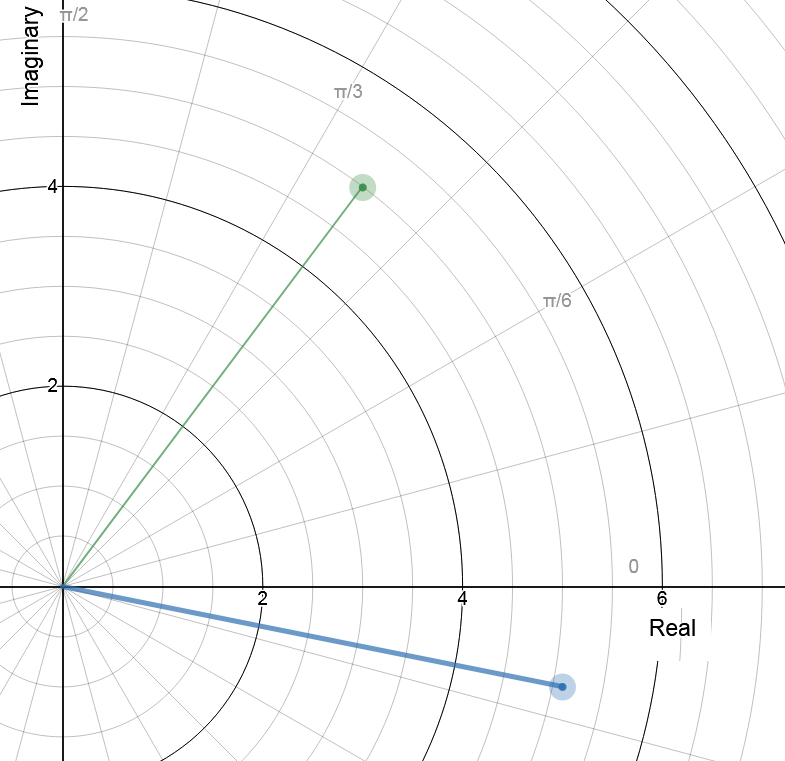
\includegraphics[scale=0.5]{Figur 1.png}
                  \end{center}

          \end{enumerate}
          \item \begin{enumerate}
                \item Med radien 5 och vinkeln $\pi/3$ så 
                skrivs den som $5e^{i\pi/3}$

                \item $$5cos(\pi/3)+i5sin(\pi/3)=\frac{5}{2}+i\frac{5\sqrt{3}}{2}$$
          \end{enumerate}

          \item denna kan skrivas om som 
          $z^2-6z+13=0$ vilket är en simpel andragradsekvation som
          kan lösas med pq-formeln 
          $$-\frac{-6}{2}\pm\sqrt{(\frac{-6}{2})^2-13}=3\pm\sqrt{-4}=3\pm 2i$$
          
          Grafiskt kan man se detta som två ställen där talen convergerar.
          Runt de områderna är dom nära noll, och presis vid $3\pm 2i$ är 
          transformeras den till noll punkten.
          \begin{center}
                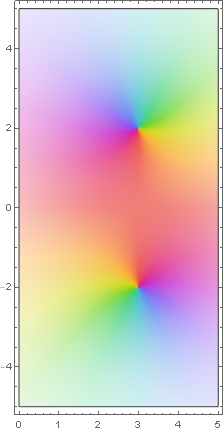
\includegraphics[scale=0.6]{Figur 2.png}
          \end{center}
          \item 
          $$\frac{10(1-2i)}{1+2i(1-2i)}=\frac{10-20i}{1+4}=2-4i$$

          \item För att utföra detta skrivs formen om till a+bi form.
          $$\frac{(2-3i)(1-ai)}{(1+ai)(1-ai)}=\frac{2-2ai-3i-3a}{1+a^2}=\frac{2-3a}{1+a^2}-\frac{2a+3}{1+a^2}i$$

          Vilket bildar en cirkel om man plottar alla värden av a, där punkten
          2-3i är där a=0 och där negativa a bildar den övre-högra delen av cirkeln
          medans positiva ger dom nere till vänster.
          Interestant att påpeka hur tvåorna och treorna i ekvationen
          verkar korrelera med där dess intersektion. Gränsvärdet
          när a närmar sig oändlighet eller minus oändlighet är 0.
          \begin{center}
                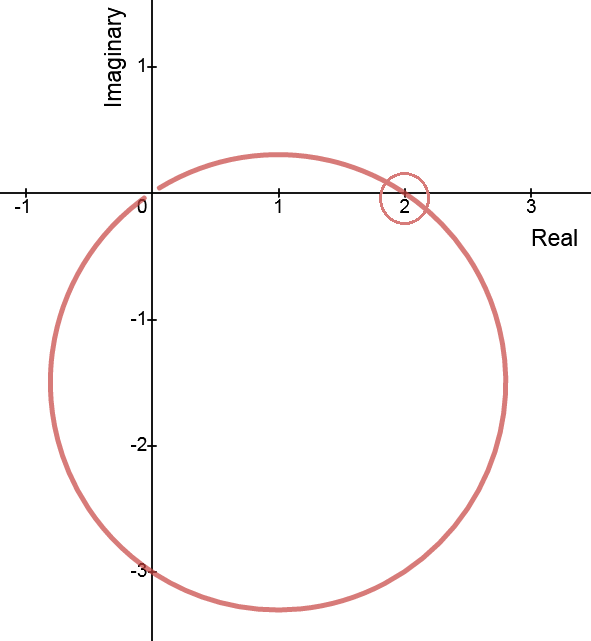
\includegraphics[scale=0.55]{Figur 3.png}
          \end{center}

          Frågan är, vid vilket a skär den reella linjen d.v.s 2?
          Man tar man ekvationen och sätter att den imaginära delen är 0.
          $$-\frac{2a+3}{1+a^2}i=0\Rightarrow -2a=3\Rightarrow a=-3/2$$

          \item 
          $$z^3=r^3e^{3(\theta+2\pi n)}$$
          
          27i ligger vid vinkeln $\pi/2$ med radien 27. Då får man att
          
          $$z^3=27e^{\frac{\pi}{2}+2\pi n}\Rightarrow z=3e^{\pi/6+2\pi n/3}$$

          Lösningarna är alltså
          $$z_1=3e^{\pi/6}$$
          $$z_1=3e^{5\pi/6}$$
          $$z_1=3e^{9\pi/6}=-3i$$
          
          Här är en illustration över lösningarna. "Singulariteterna" visar på där
          x och y ko-ordinaterna är input till funktionen och färgen visar outputten.
          Runt rötterna som tidigare räknats ut drar sig outputen närmare noll ju närmare
          rötterna dom kommer i inputten.

          Eftersom att dom är alla lika långt bort från origon så hamnar dom även på
          en cirkel med radien 3 runt origon.

          \begin{center}
                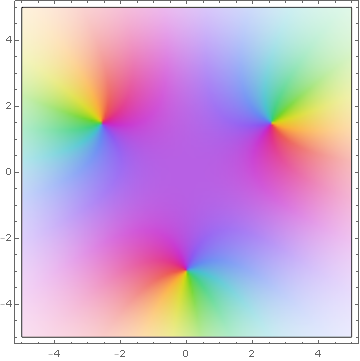
\includegraphics[scale=0.5]{Figur 5.png}
          \end{center}

          \item $$z_1=2e^{-5\pi/18}$$
            $$z_2=3e^{4\pi/18}$$
          $$arg(3z_1\cdot 2z_2)=arg(2\cdot 3e^{-5\pi/18+4\pi/18})=arg(6e^{-\pi/18})=-\frac{\pi}{18}$$

          Detta är logiskt då vi tar ett tal med vinkeln 40 grader minus ett med vinkeln 50 grader,
          så att summan blir minus 10 grader.

          \item Vi vet att en rot är 0.5, så med hjälp av faktorisering 
          
          $$(x-0.5)(x^2-6x-16)$$
          
          Och sedan löses andragradsekvationen

          $$(x-0.5)(x-8)(x+2)$$

          Vilket kan konstateras grafiskt

          \begin{center}
                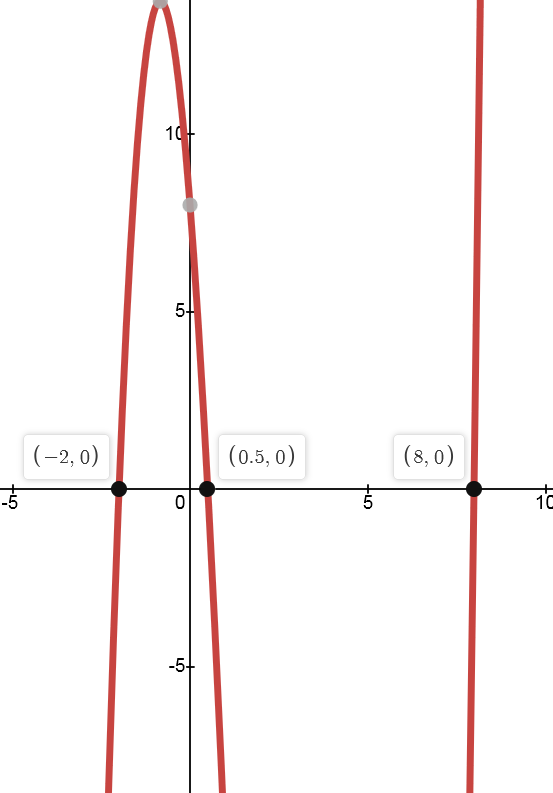
\includegraphics[scale=0.4]{Figur 4.png}
          \end{center}

\end{enumerate}
\end{document}